\section{Ergebnisse}\label{kap:5}
\subsection{Portfoliodatensatz}
Nach Abschluss aller in Kapitel \ref{sec:createportfolio} beschriebenen Schritte wurde ein realistisches Portfolio von Hypotheken-Immobilien erstellt.
Abbildung \ref{fig:hypothekenportfolio} zeigt die resultierende Distribution der Datenpunkte auf der Karte Bayerns.

\begin{figure}[htbp]
    \centering
    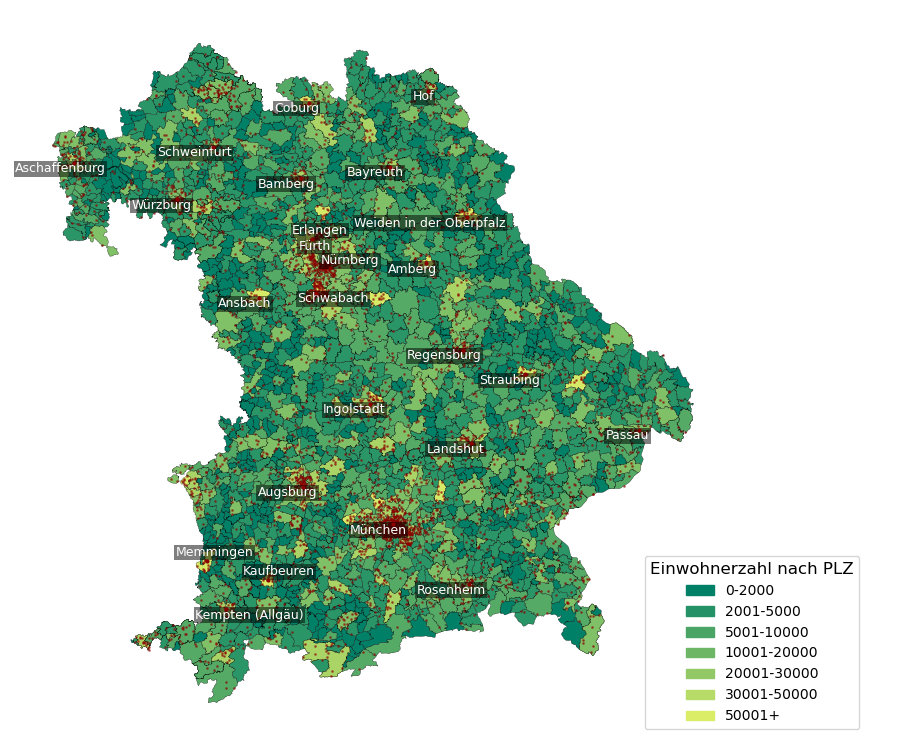
\includegraphics[width=1.2\textwidth]{figures/bayern_por_pop.png} 
    \caption{Datenpunktverteilung im Hypothekenportfolio Bayern. Quelle: Eigene Darstellung}
    \label{fig:hypothekenportfolio}
\end{figure}
\FloatBarrier
\clearpage
Abbildung \ref{fig:bayernflut} präsentiert das Resultat dieser Vereinheitlichung der Datenpunkte auf der Karte Bayerns mit den Hochwasserrisikogebieten.

\begin{figure}[htbp]
    \centering
    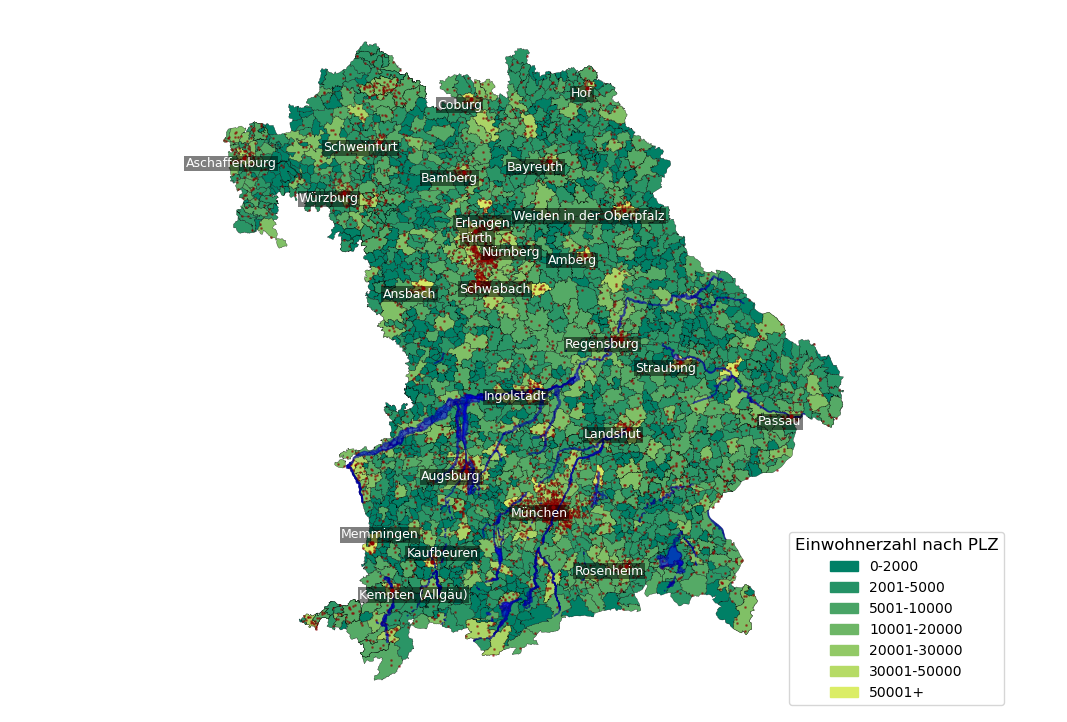
\includegraphics[width=1.2\textwidth]{figures/bayern_flut.png} 
    \caption{Visualisierung historischer Hochwasserereignisgebiete und Verteilung des Darlehensportfolios in Bayern. Quelle: Eigene Darstellung}
    \label{fig:bayernflut}
\end{figure}
\FloatBarrier
\clearpage
Als Ergebnis entstand ein umfassender Datensatz, dessen Grundlage die in Tabelle \ref{tab:objekt-variablen} beschriebenen Objektvariablen bilden.
\begin{table}[htbp]
    \centering
    \small
    \caption{Übersicht über das Hypothekenportfolio und die relevanten Objekt-Variablen}
    \label{tab:objekt-variablen}
    \begin{tabularx}{1.0\textwidth}{>{\raggedright\arraybackslash}X >{\raggedright\arraybackslash}X}
        \toprule
        \textbf{Objekt-Variablen} & \textbf{Erklärung} \\
        \midrule
        ID & Identifikationsnummer \\
        \addlinespace
        Ort & Ort der Immobilie \\
        \addlinespace
        Landkreis & Landkreis der Immobilie \\
        \addlinespace
        Latitude & Breitengrad der Immobilie zur genauen Lokalisierung \\
        \addlinespace
        Longitude & Längengrad der Immobilie zur genauen Lokalisierung \\
        \addlinespace
        GEB\_Q & Hochwasser Ergebnis \\
        \addlinespace
        AEP & Jährliche Überschreitungswahrscheinlichkeit \\
        \addlinespace
        Überschwemmung Tiefe & Tiefe der Überschwemmung an dem Punkt \\
        \addlinespace
        Überschwemmungsrisiko Stufe & Stufe des Überschwemmungsrisikos \\
        \addlinespace
        Energieklasse & Energieeffizienzklasse der Immobilie \\
        \addlinespace
        Quadratmeterpreise & Preis pro Quadratmeter der Immobilie \\
        \addlinespace
        Wohnfläche & Gesamte Wohnfläche der Immobilie in Quadratmetern \\
        \addlinespace
        Aktueller Immobilienwert & Der aktuelle Wert der Immobilie \\
        \addlinespace        Aktuelles LTV & Aktuelles Verhältnis von Darlehen zu Wert (Loan-to-Value) \\
        \bottomrule
    \end{tabularx}
\end{table}
\FloatBarrier
Der Datensatz umfasst 3853 Datenpunkte, verteilt auf 1522 Orte und 71 Landkreise in Bayern. Die Verteilung der Energieklassen der Datenpunkte stimmt mit der bayerischen Energieklassenverteilung laut Tabelle \ref{tab:epc_bayern} überein. Ähnlich orientiert sich die LtV-Verteilung an Tabelle \ref{tab:beleihungsauslauf2023}.
\begin{table}[htbp]
    \centering
    \caption{Statistische Zusammenfassung der Hypothekendaten}
    \label{tab:hypothekenuberblick}
    \small
    \begin{tabularx}{\textwidth}{>{\raggedright\arraybackslash}m{3.5cm}*{5}{>{\centering\arraybackslash}X}}
    \toprule
    Metrik & Mean & Median & Min & Max & Std \\
    \midrule
    Preis/m² & 2.458,57 & 2.032,01 & 685,48 & 5.297,69 & 1.320,59 \\
    Wohnfläche & 114,40 & 111,78 & 80,00 & 168,23 & 29,14 \\
    Akt. Immnwert & 281.726,31 & 229.186,05 & 54.838,79 & 889.649,95 & 173.681,59 \\
    Akt. LtV & 0,5978 & 0,6000 & 0,4200 & 0,7500 & 0,1012 \\
    Darlehenbetrag & 168.148,10 & 136.034,00 & 26.368,90 & 662.763,36 & 108.638,21 \\
    \bottomrule
    \end{tabularx}
\end{table}

\subsection{Physische Risiko}
Die Hochwasserrisikostufen im erstellten Portfolio sind wie folgt verteilt: 1 hohes, 17 mittlere, 12 niedrige und 3823 sehr niedrige Risiken. Diese Risikostufeverteilung wird in Abbildung \ref{fig:riskostufe} graphisch dargestellt und visualisiert.
\begin{figure}[htbp]
    \centering
    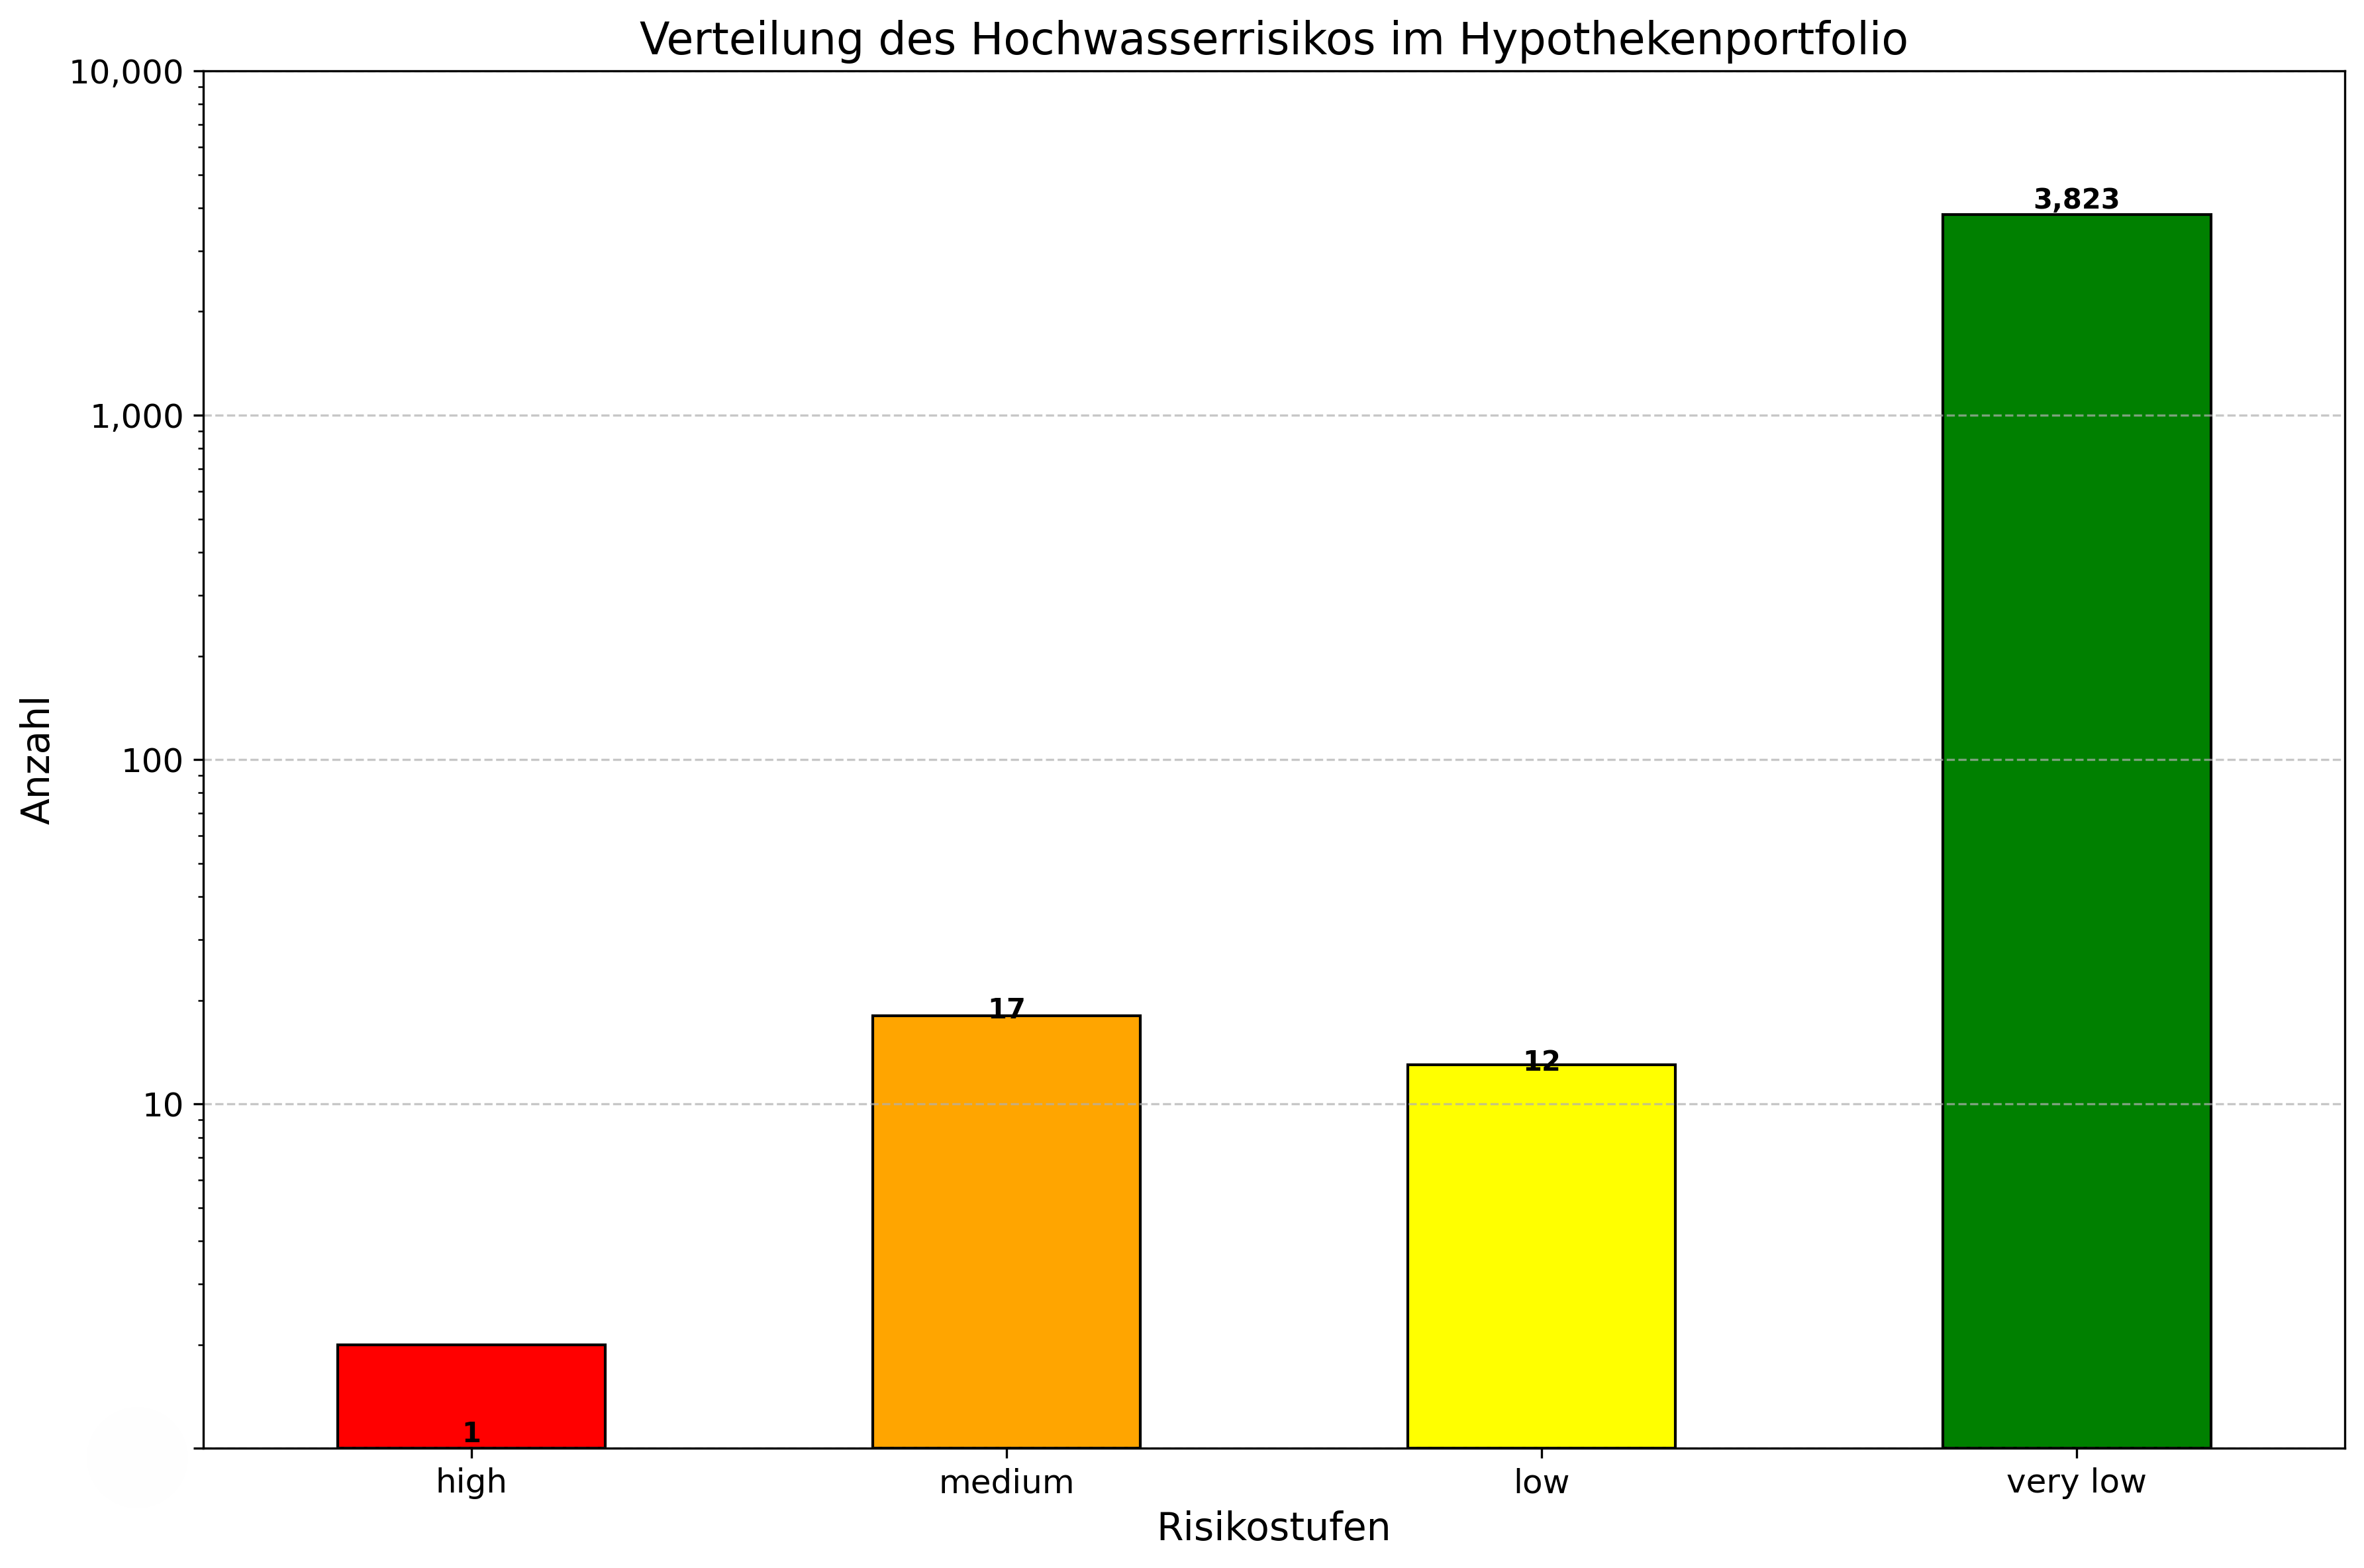
\includegraphics[width=0.8\textwidth]{figures/hochwasserrisiko_verteilung.png}
    \caption{Verteilung der Hochwasserrisikostufen im Hypothekenportfolio. Quelle: Eigene Darstellung}
    \label{fig:riskostufe}
\end{figure}
\FloatBarrier
Mittels des digitalen Geländemodells von Bayerns sowie Pegelnullpunkt und Hochwasserstand von \textcite{bayern2016hochwassernachrichtendienst} wurde die Überflutungstiefe bestimmt. Dies betrifft Datenpunkte in den Kategorien hoch, mittel und niedrig.

Nach der Berechnung der Überflutungstiefe kann durch den Vergleich mit der Schadenfunktion in Abbildung \ref{fig:damage_curve2} der entsprechende Schadensfaktor ermittelt werden. Basierend auf diesem Schadensfaktor lässt sich mithilfe der Gleichung \ref{eq:schaden} der Immobilienschaden quantifizieren. Die Resultate dieser Berechnungen für den Immobilienschaden werden anschließend in Abbildung \ref{fig:schadenwert} grafisch dargestellt.
\begin{figure}[htbp]
    \centering
    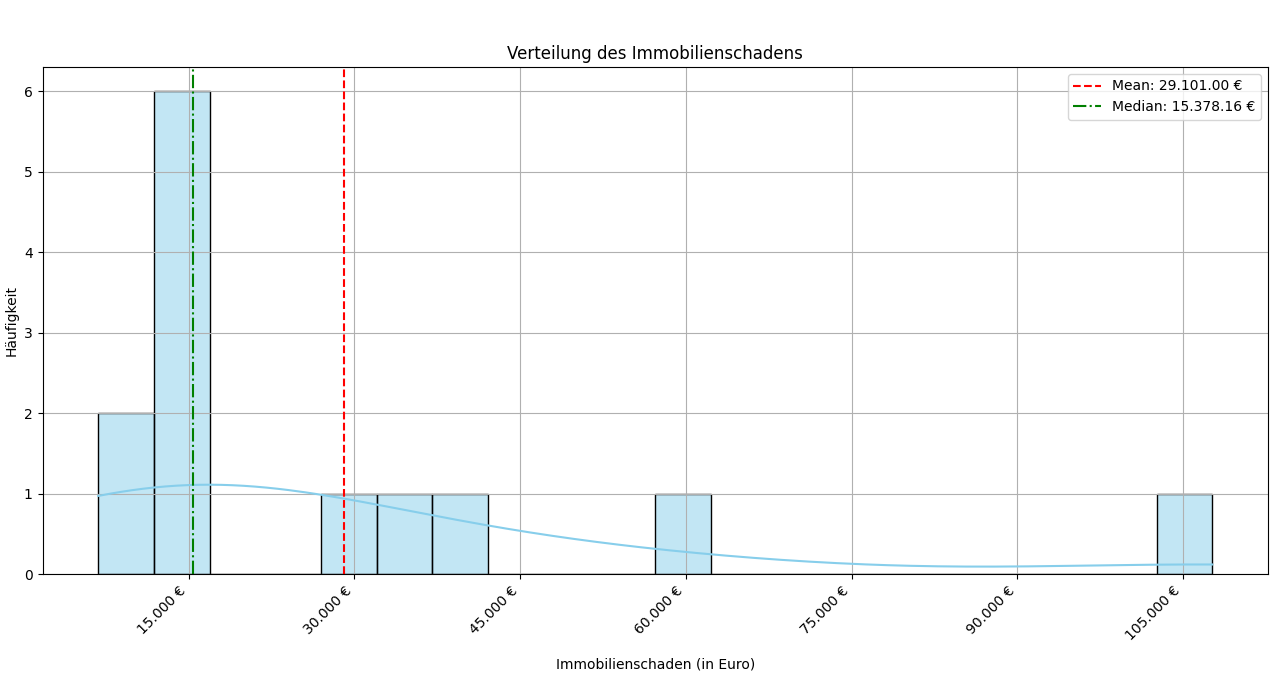
\includegraphics[width=\textwidth]{figures/flutschaden.png}
    \caption{Verteilung des Immobilienschaden im Hypothekenportfolio. Quelle: Eigene Darstellung}
    \label{fig:schadenwert}
\end{figure}
\FloatBarrier
In der folgenden Abbildung \ref{fig:schadenereignis} wird der prozentuale Gesamtschadenwert im Vergleich zum Gesamtimmobilienwert im Falle des Eintritts eines Schadensereignisses dargestellt. Abbildung \ref{fig:schadenereignis_jahr} zeigt den prozentualen Gesamtschadenwert im Vergleich zum Gesamtimmobilienwert, wenn ein Schadensereignis innerhalb eines Jahres eintritt.\begin{figure}[H]
    \centering
    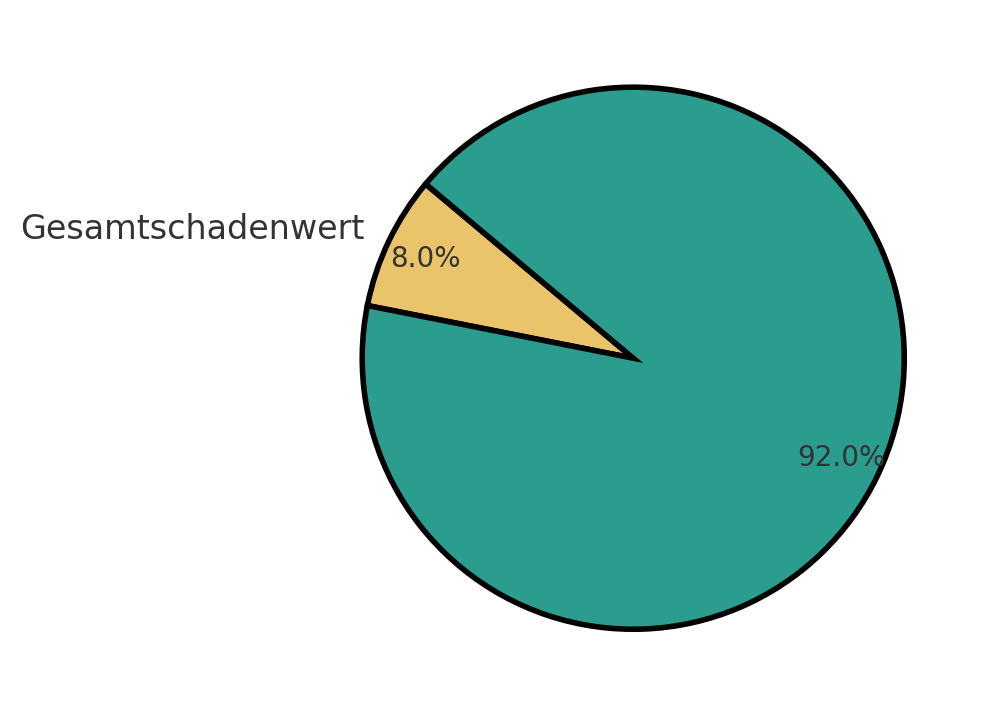
\includegraphics[width=0.45\textwidth]{figures/roundchartsloss.png}
    \caption{Prozentualer Gesamtschaden am Immobilienwert im Schadensfall}
    \label{fig:schadenereignis}
\end{figure}

\begin{figure}[H]
    \centering
    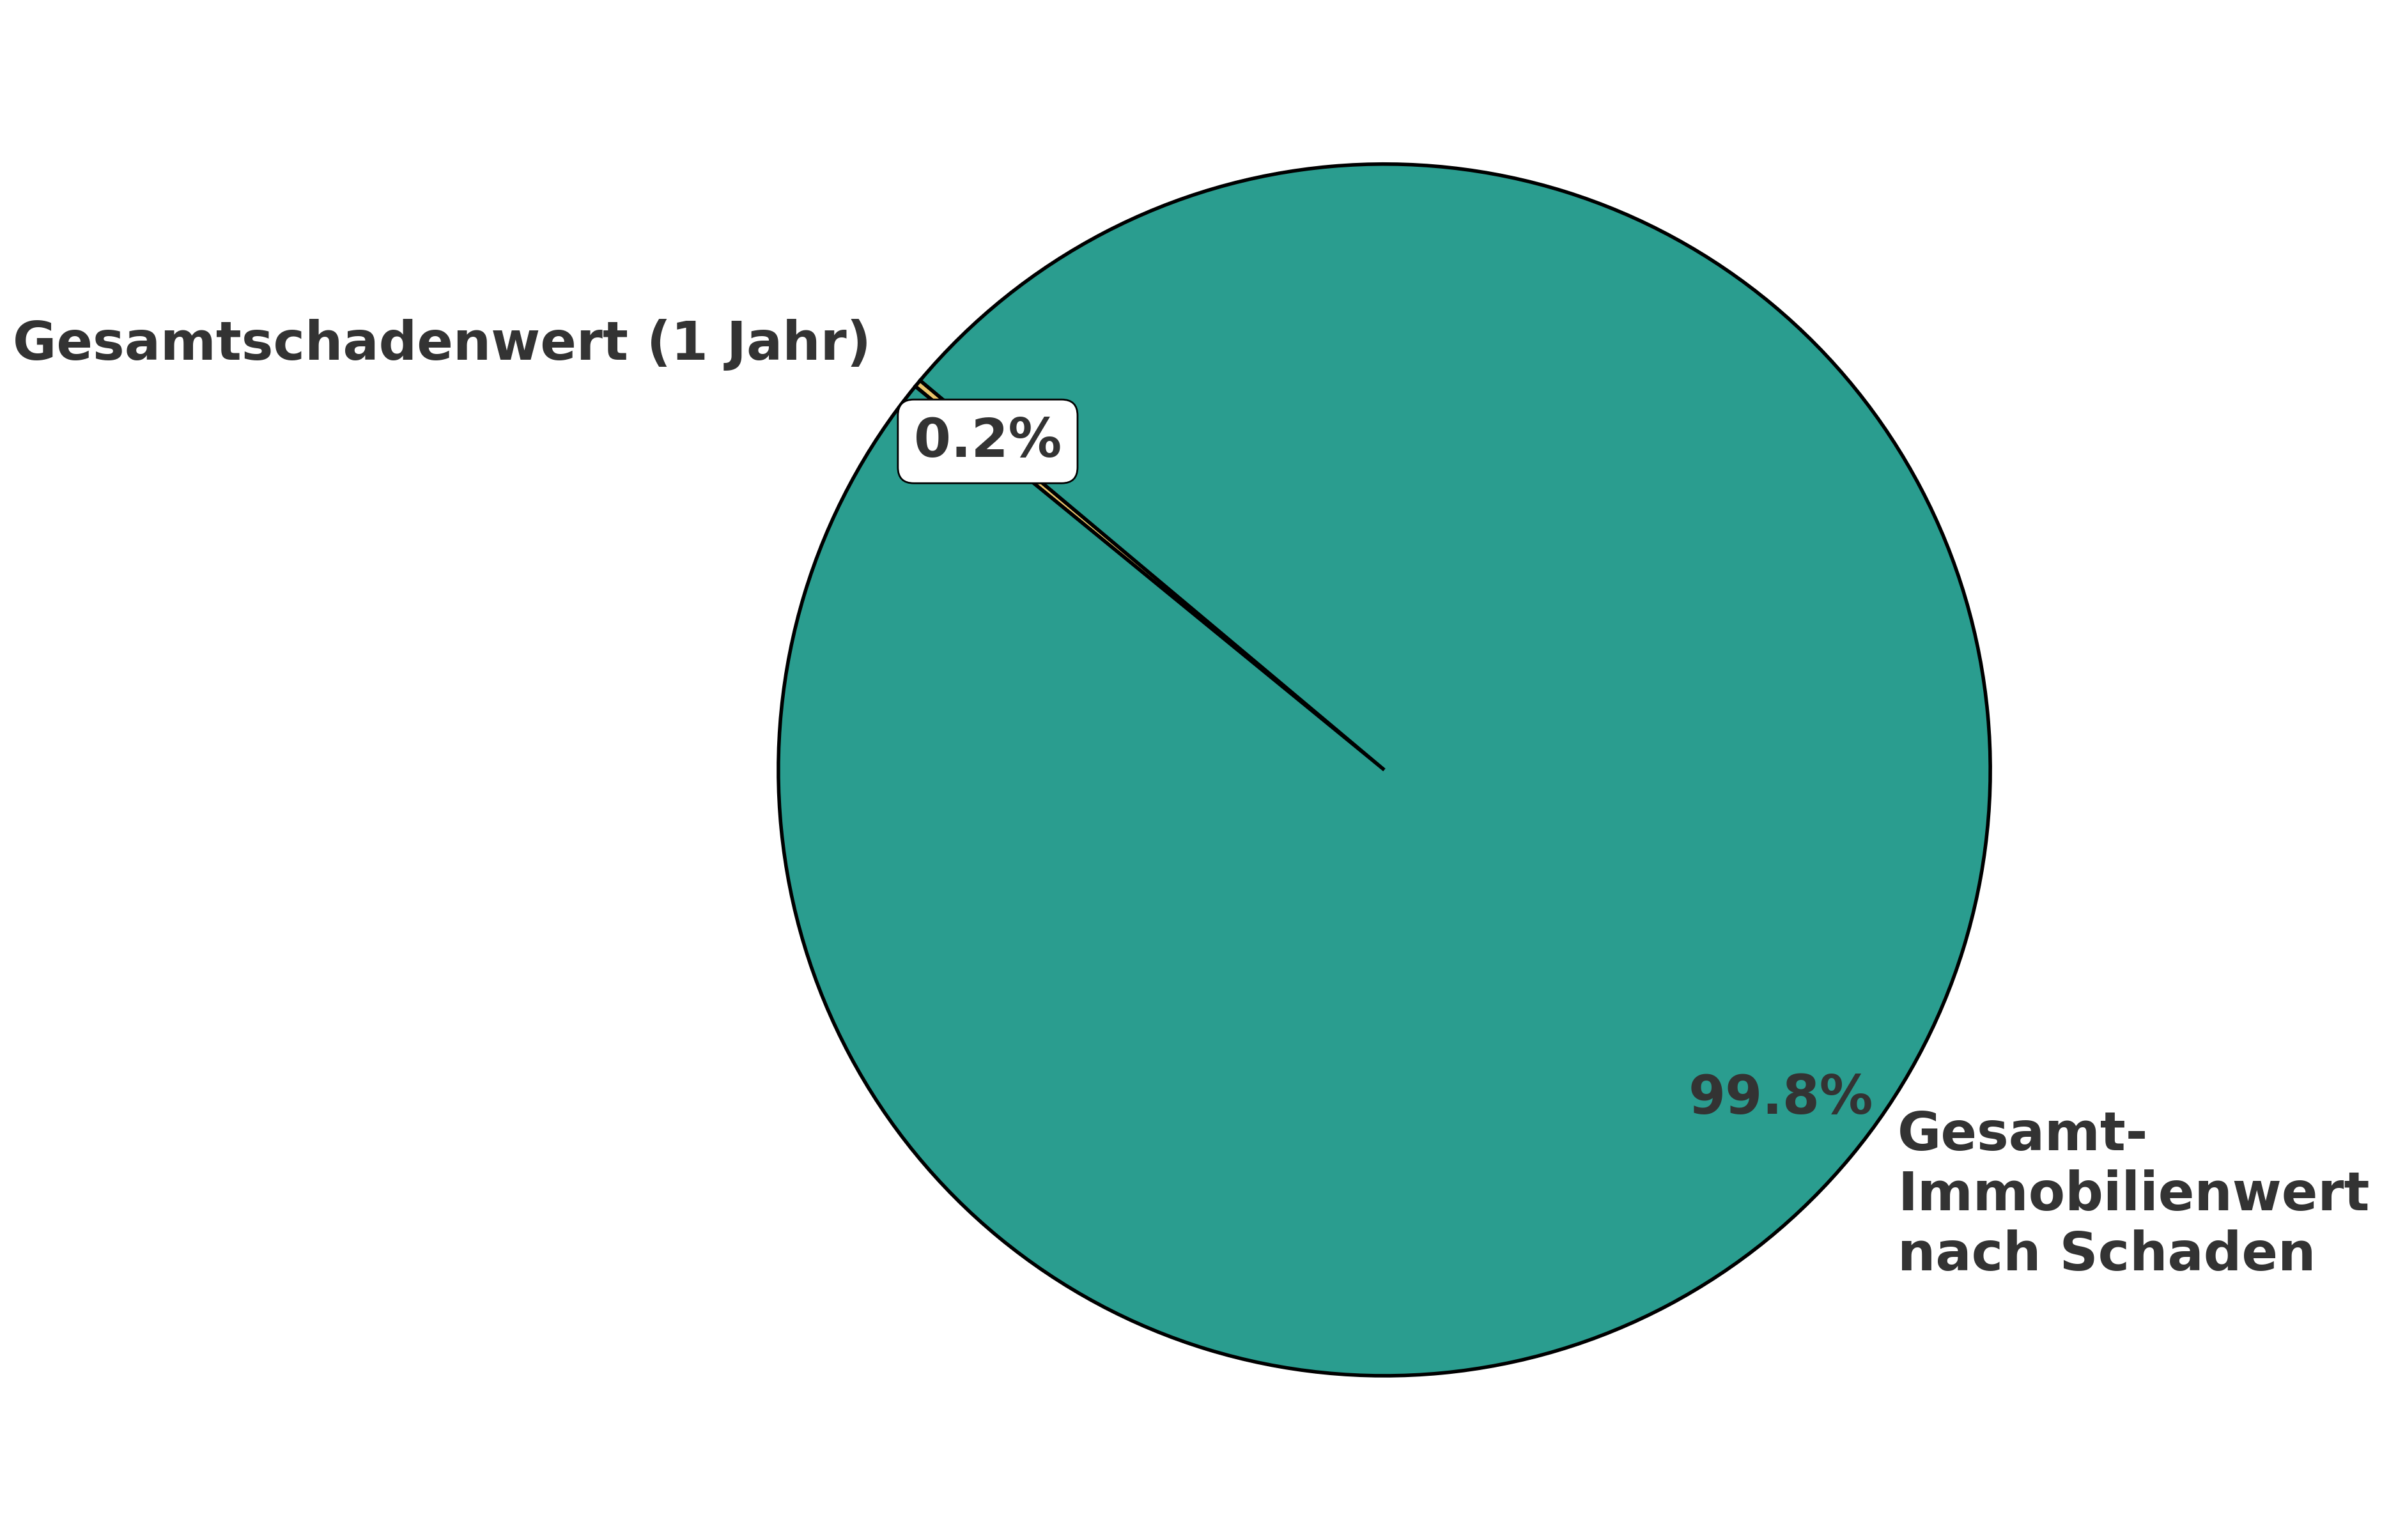
\includegraphics[width=0.45\textwidth]{figures/roundchartloss1year.png}
    \caption{Prozentualer Gesamtschaden am Immobilienwert im Jahresschadensfall}
    \label{fig:schadenereignis_jahr}
\end{figure}

In der folgenden Tabelle \ref{tab:rwa_anderung} sind die Veränderungen des Beleihungsauslaufs und des Risikogewichts infolge eines Schadensereignisses dargestellt.
\begin{table}[htbp]
    \centering
    \caption{Übersicht der Änderungen von LtV und RWA nach Schadensereignis}
    \label{tab:rwa_anderung}
    \footnotesize 
    \begin{tabularx}{\textwidth}{>{\raggedright\arraybackslash}m{1.0cm} *{4}{>{\centering\arraybackslash}m{1.3cm}} >{\raggedleft\arraybackslash}m{2.0cm} >{\raggedleft\arraybackslash}m{2.0cm} >{\centering\arraybackslash}m{1.0cm}}
    \toprule
    ID & Akt. LtV & Neu LtV & Akt. RW & Neu RW & \makecell{Akt. \\ RWA / €} & \makecell{Neu \\ RWA / €} & \(\Delta\) RWA \\
    \midrule
    2633 & 0.44 & 0.67 & 0.20 & 0.30 & 26.843,55 & 40.265,32 & 0,50 \\
    3688 & 0.48 & 0.50 & 0.20 & 0.25 & 38.995,87 & 48.744,84 & 0,25 \\
    2635 & 0.52 & 0.60 & 0.25 & 0.30 & 60.503,46 & 72.604,15 & 0,20 \\
    3376 & 0.56 & 0.67 & 0.25 & 0.30 & 36.661,73 & 43.994,08 & 0,20 \\
    2634 & 0.74 & 0.77 & 0.30 & 0.30 & 57.615,57 & 57.615,57 & 0,00 \\
    2961 & 0.65 & 0.69 & 0.30 & 0.30 & 117.890,11 & 117.890,11 & 0,00 \\
    2666 & 0.44 & 0.45 & 0.20 & 0.20 & 63.261,10 & 63.261,10 & 0,00 \\
    3358 & 0.70 & 0.76 & 0.30 & 0.30 & 40.379,53 & 40.379,53 & 0,00 \\
    3716 & 0.52 & 0.55 & 0.25 & 0.25 & 32.263,95 & 32.263,95 & 0,00 \\
    3719 & 0.67 & 0.72 & 0.30 & 0.30 & 45.931,46 & 45.931,46 & 0,00 \\
    3775 & 0.55 & 0.57 & 0.25 & 0.25 & 31.190,40 & 31.190,40 & 0,00 \\
    3776 & 0.54 & 0.55 & 0.25 & 0.25 & 61.807,26 & 61.807,26 & 0,00 \\
    3778 & 0.54 & 0.59 & 0.25 & 0.25 & 43.608,49 & 43.608,49 & 0,00 \\
    \midrule
    Sum & & & & & 656.952,48 € & 699.556,26 € &  \\
    \bottomrule
    \end{tabularx}
\end{table}









\subsection{Transitionsrisiko}
Abbildung \ref{fig:endpreis_energie} zeigt das Ergebnis der Berechnungen des Endpreises für Energie, basierend auf den NGFS-Szenarien, unter Berücksichtigung der Mehrwert- und Energiesteuern in vier NGFS-Szenarien: Netto-Null, Ungeordnet (Disorderly), Unter 2°C (Below 2 Degrees) und Aktuelle Richtlinien (Current Policies).

\begin{figure}[htbp]
    \centering
    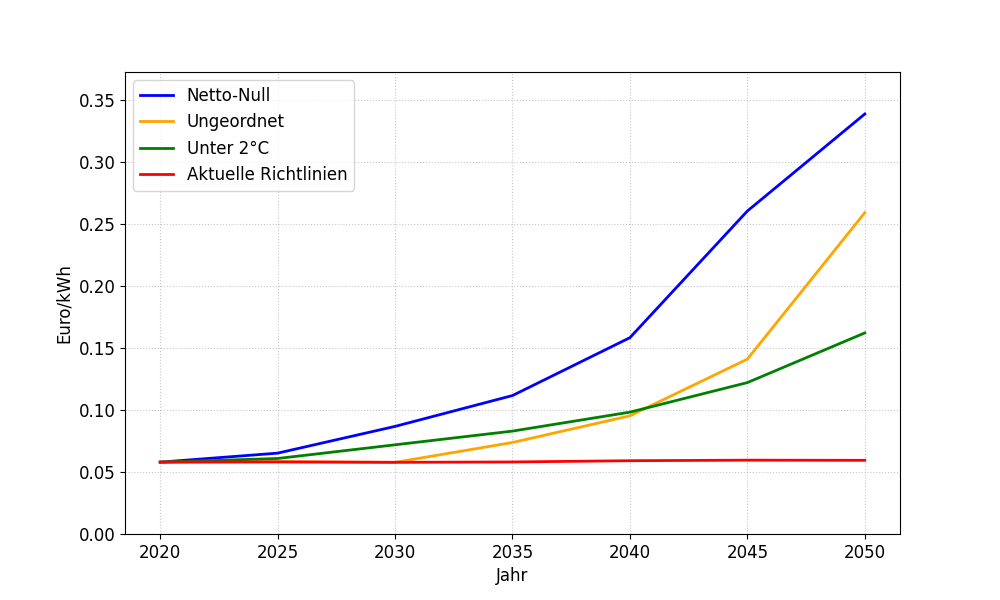
\includegraphics[width=\textwidth]{figures/endpreis.png}
    \caption{Endpreis der Energie mit Mehrwert- und CO2-Steuern nach NGFS-Szenarien. Quelle: Eigene Darstellung}
    \label{fig:endpreis_energie}
\end{figure}
\FloatBarrier

Auf Grundlage des zuvor berechneten Endenergiepreises und der Formel aus Abschnitt \ref{sec:endenfkt} wurde die absolute Wertänderung der Immobilien ermittelt. Diese Berechnungen wurden für Häuser mit Energieeffizienzklassen unterhalb von A und A+ vorgenommen. Die Analysen ergaben Daten zur jährlichen absoluten Werteentwicklung dieser Immobilien. Zudem wurden verschiedene Szenarien betrachtet.und der Formel aus Abschnitt \ref{sec:endenfkt} wurde die absolute Wertänderung der Immobilien ermittelt. Diese Berechnungen wurden für Häuser mit Energieeffizienzklassen unterhalb von A und A+ vorgenommen. Die Analysen ergaben Daten zur jährlichen absoluten Werteentwicklung dieser Immobilien. Zudem wurden verschiedene Szenarien betrachtet.

Die folgenden Abbildungen zeigen die absoluten Immobilien-Wertsveränderungen in Abhängigkeit von Zeit und Szenario.

\begin{figure}[htbp]
    \centering
    \begin{subfigure}[b]{0.48\textwidth}
        \centering
        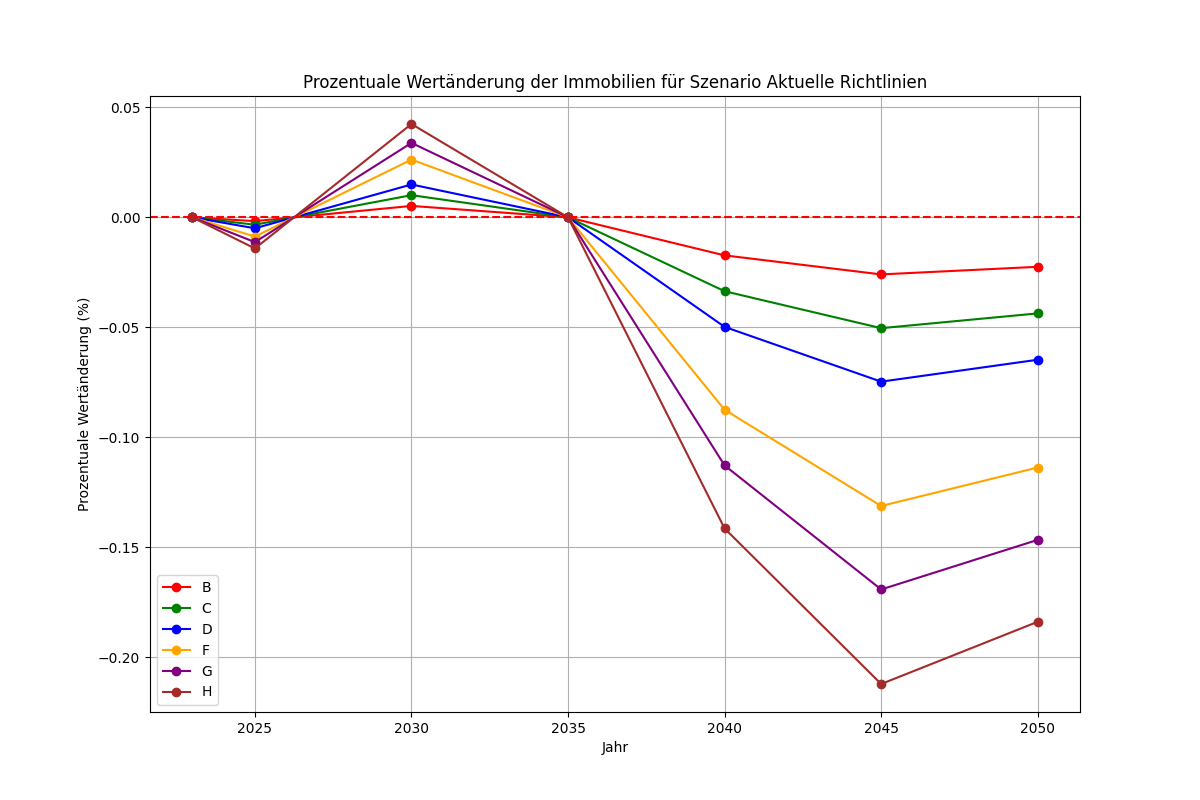
\includegraphics[width=\textwidth]{figures/Aktuelle Richtlinien_percentage_change_plot.png}
        \caption{Prozentuale Wertänderung der Immobilien im Szenario Aktuelle Richtlinien.}
        \label{fig:aktuelle_richtlinien}
    \end{subfigure}
    \hfill
    \begin{subfigure}[b]{0.48\textwidth}
        \centering
        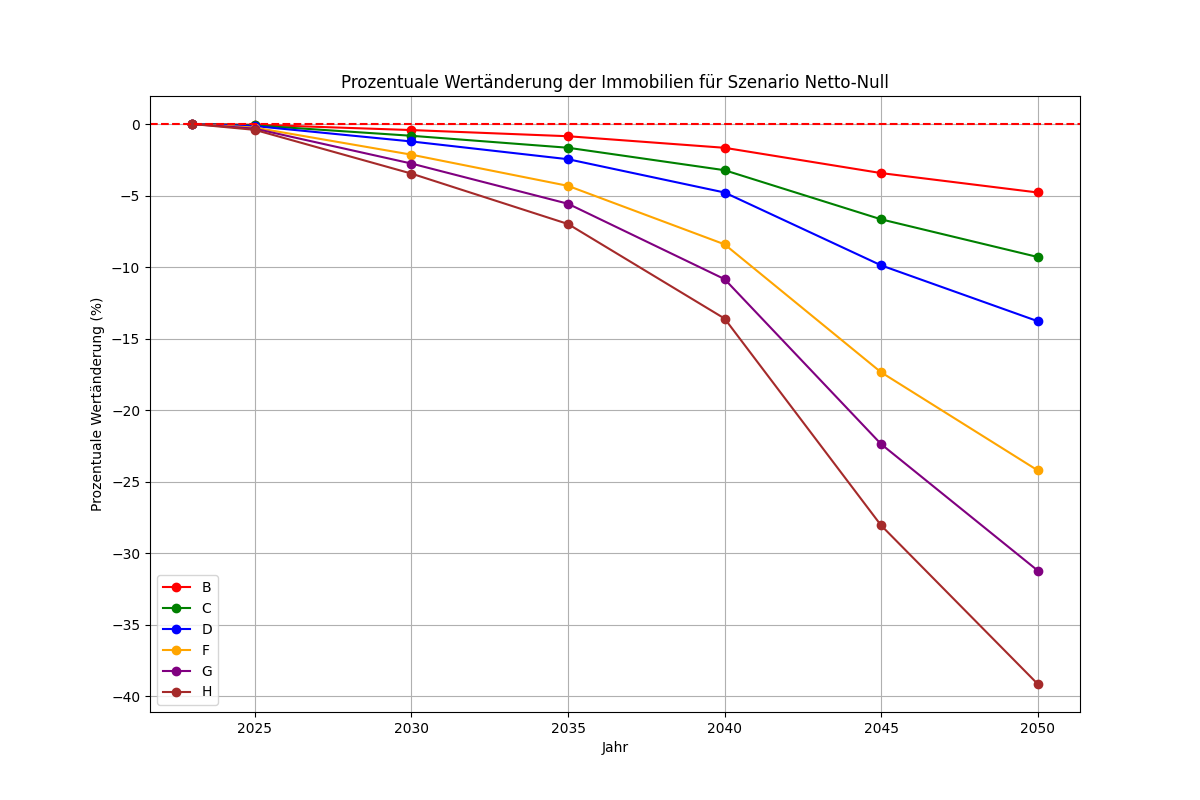
\includegraphics[width=\textwidth]{figures/Netto-Null_percentage_change_plot.png}
        \caption{Prozentuale Wertänderung der Immobilien im Szenario Netto-Null.}
        \label{fig:netto_null}
    \end{subfigure}
    
    \vspace{1em}
    
    \begin{subfigure}[b]{0.48\textwidth}
        \centering
        \includegraphics[width=\textwidth]{figures/Unter 2°C_percentage_change_plot.png}
        \caption{Prozentuale Wertänderung der Immobilien im Szenario Unter 2°C.}
        \label{fig:unter_2c}
    \end{subfigure}
    \hfill
    \begin{subfigure}[b]{0.48\textwidth}
        \centering
        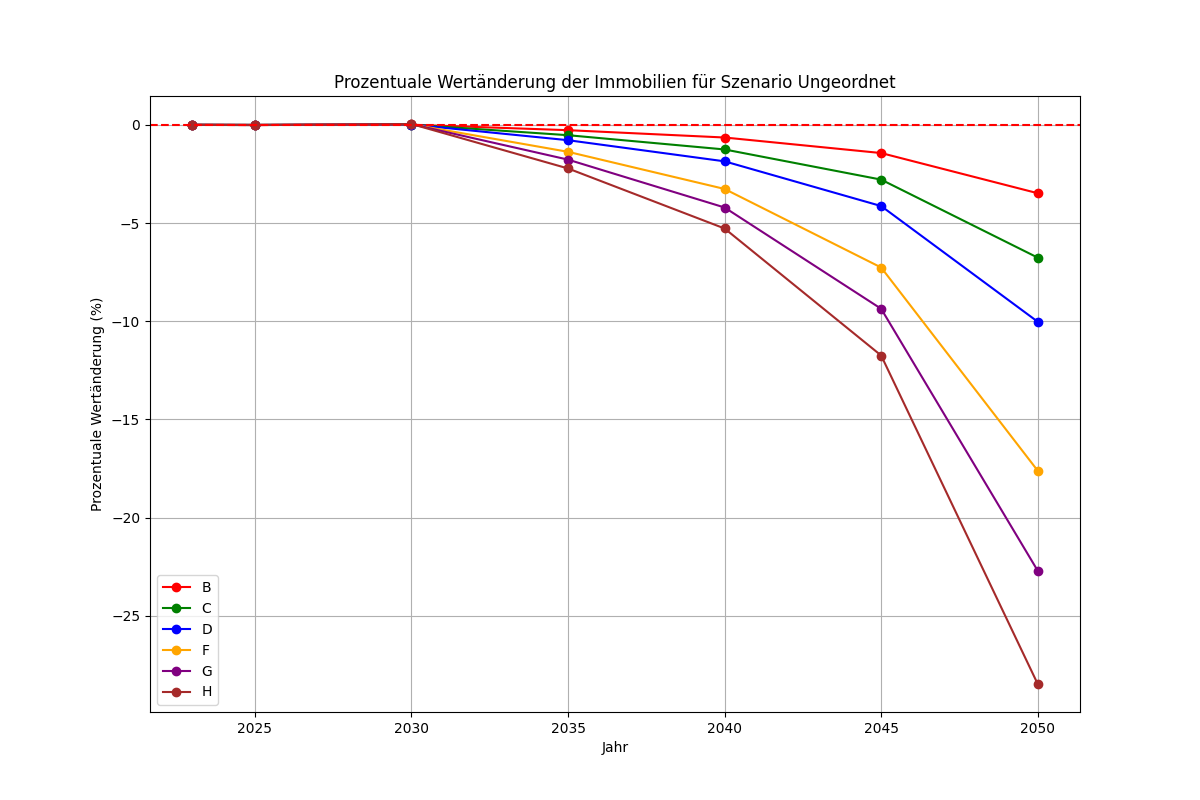
\includegraphics[width=\textwidth]{figures/Ungeordnet_percentage_change_plot.png}
        \caption{Prozentuale Wertänderung der Immobilien im Szenario Ungeordnet.}
        \label{fig:ungeordnet}
    \end{subfigure}
    \caption{Prozentuale Wertänderung der Immobilien in verschiedenen Szenarien.Quelle: Eigene Darstellung}
    \label{fig:all_scenarios}
\end{figure}

Abbildung \ref{fig:gesamt_rwa_plot} zeigt die Entwicklung der Gesamt-\acs{RWA} in verschiedenen Klimaszenarien.
\begin{figure}[htbp]
    \centering
    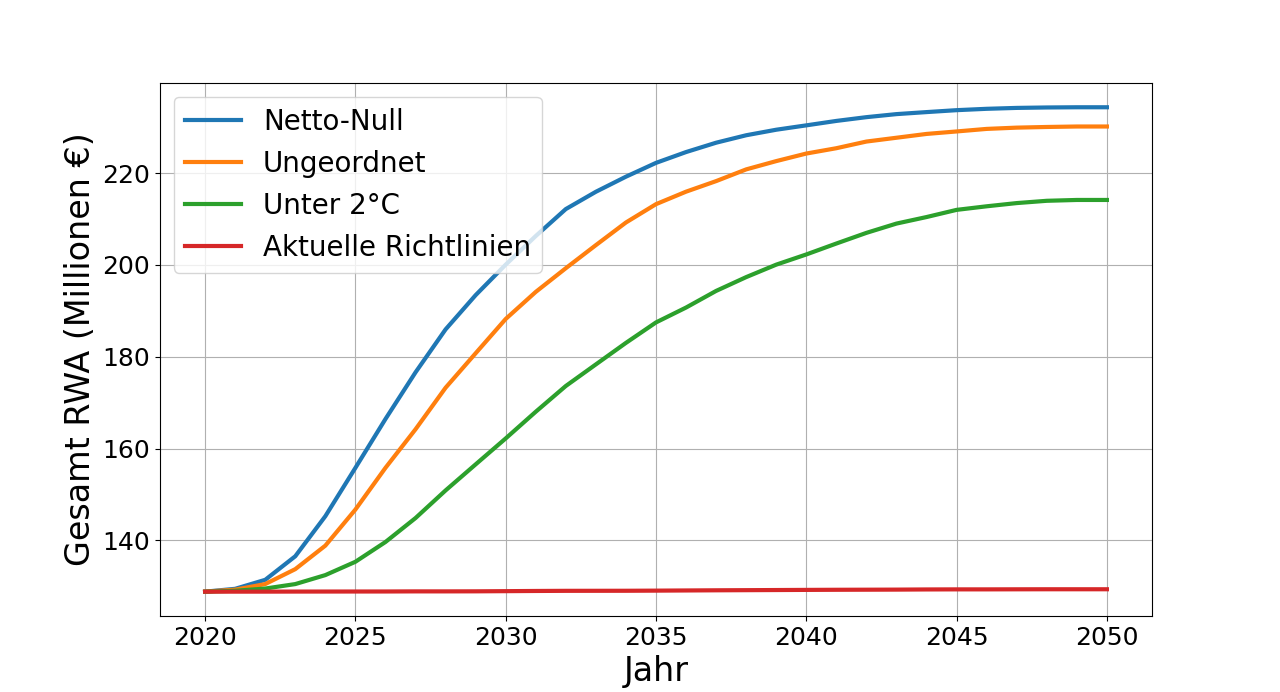
\includegraphics[width=\textwidth]{figures/gesamt_rwa_plot.png}
    \caption{Entwicklung der Gesamt-RWA in verschiedenen NGFS-Szenarien. Quelle: Eigene Darstellung}
    \label{fig:gesamt_rwa_plot}
\end{figure}
\FloatBarrier